%------------------------------------------------

\begin{frame}
  \frametitle{\'Etude d'impact sur une tâche temps-réel}
  \framesubtitle{Méthodologie}
  \begin{enumerate}
  \item<1-> Métriques
    \begin{itemize}
    \item Temps d'exécution
    \item Bande passante utilisée sur le système
    \end{itemize}
  \item<2-> Tâches temps-réel
    \begin{itemize}
    \item Benchmark MiBench
    \item Sous-ensemble d'applications représentatives d'un système automobile
    \end{itemize}
  \item<3-> Jeu de tests
    \begin{itemize}
    \item Tâche temps-réel en isolation
    \item Tâche temps-réel vs Routino (3 instances)
    \item Tâche temps-réel vs Routino MT (3 threads)
    \end{itemize}
  \item<4> Protocole
    \begin{itemize}
    \item[$T_0$] Lancement du/des Routino(s) si nécessaire (durée $\approx$
      45-80 s)
    \item[$T_0+\Delta$] Lancement de la tâche temps-réel (durée $<$ 100 ms)
    \end{itemize}
  \end{enumerate}
\end{frame}

%------------------------------------------------

\begin{frame}
  \frametitle{\'Etude d'impact sur une tâche temps-réel}
  \framesubtitle{Impact sur le temps d'exécution}
  \begin{center}
    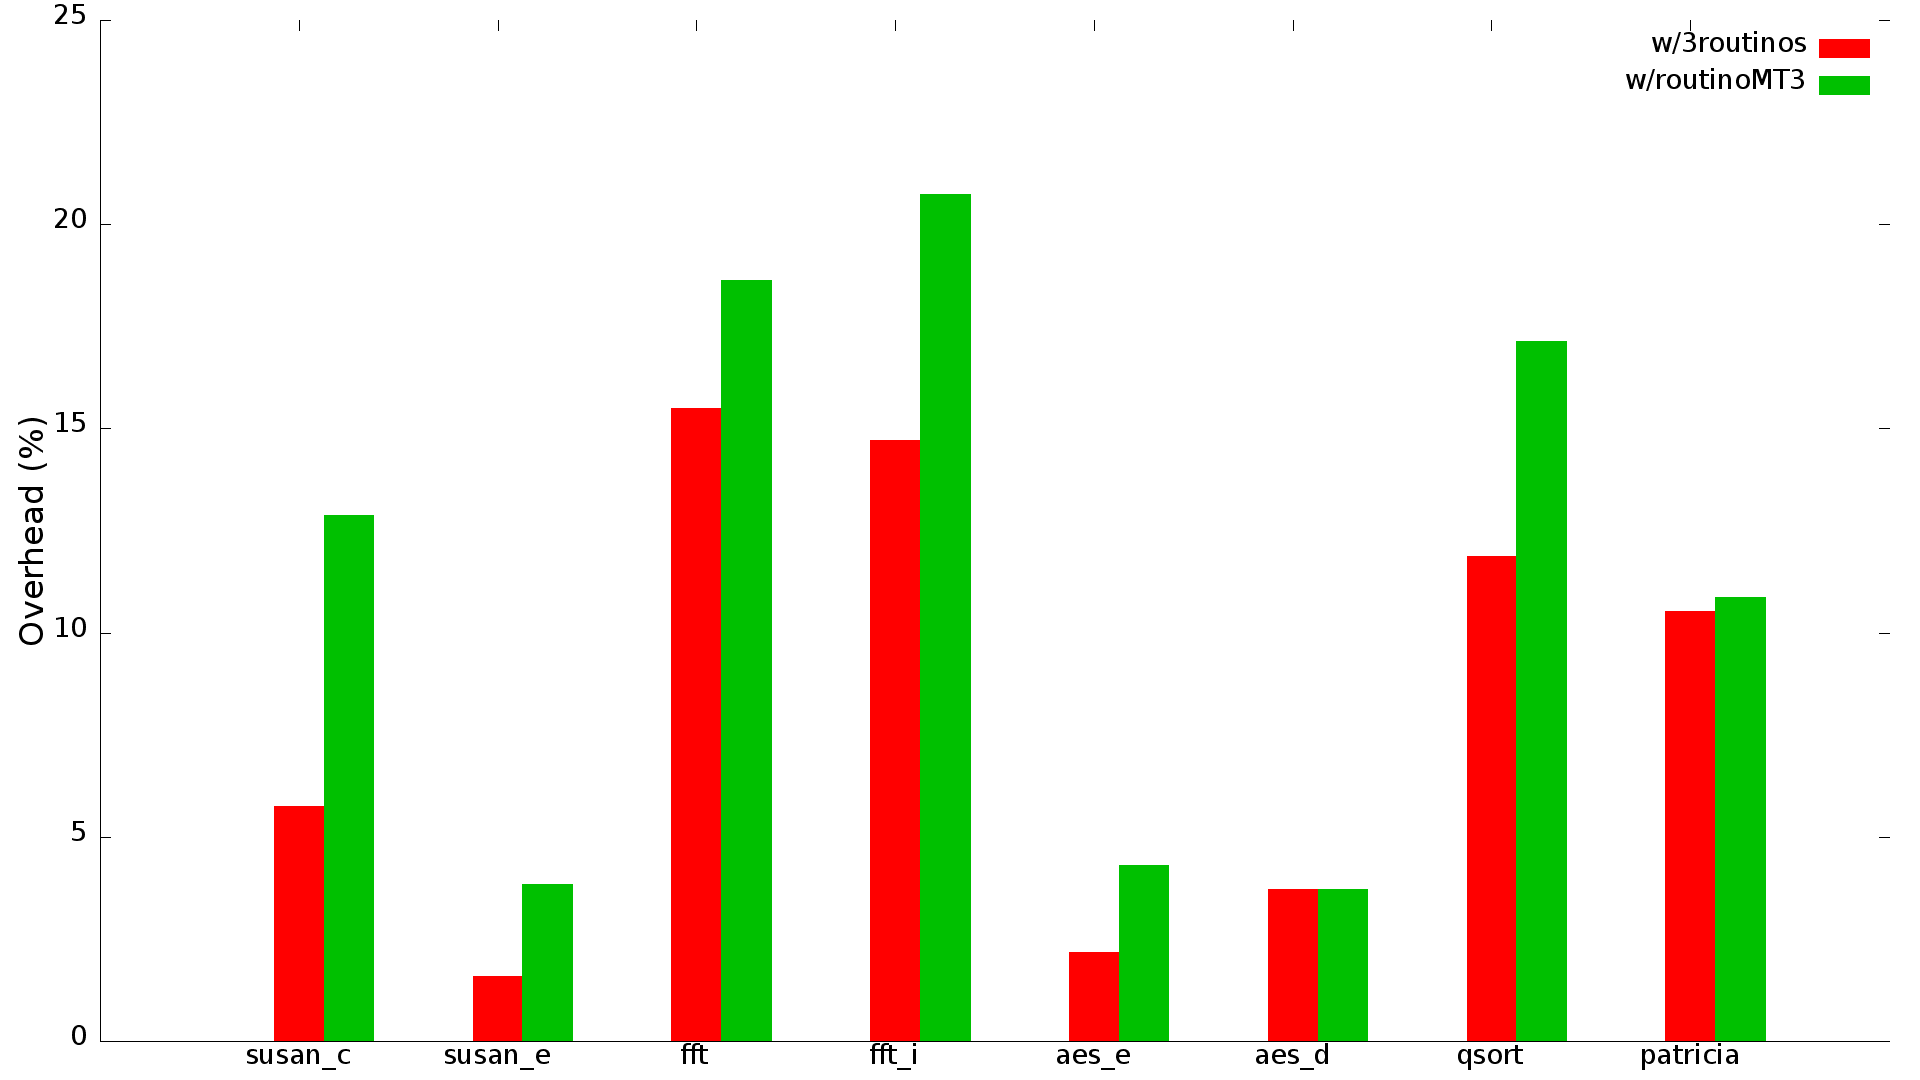
\includegraphics[scale=0.18]{include/overhead.png}
  \end{center}
  \visible<2>{
    \begin{exampleblock}{Observations}
      \begin{itemize}
      \item Augmentation de 2 à 20\% du temps d'exécution
      \item \'Ecart de surcoût non constant
      \end{itemize}
    \end{exampleblock}
  }
\end{frame}

%------------------------------------------------

\begin{frame}
  \frametitle{\'Etude d'impact sur une tâche temps-réel}
  \framesubtitle{Impact sur la bande passante}
  \begin{center}
    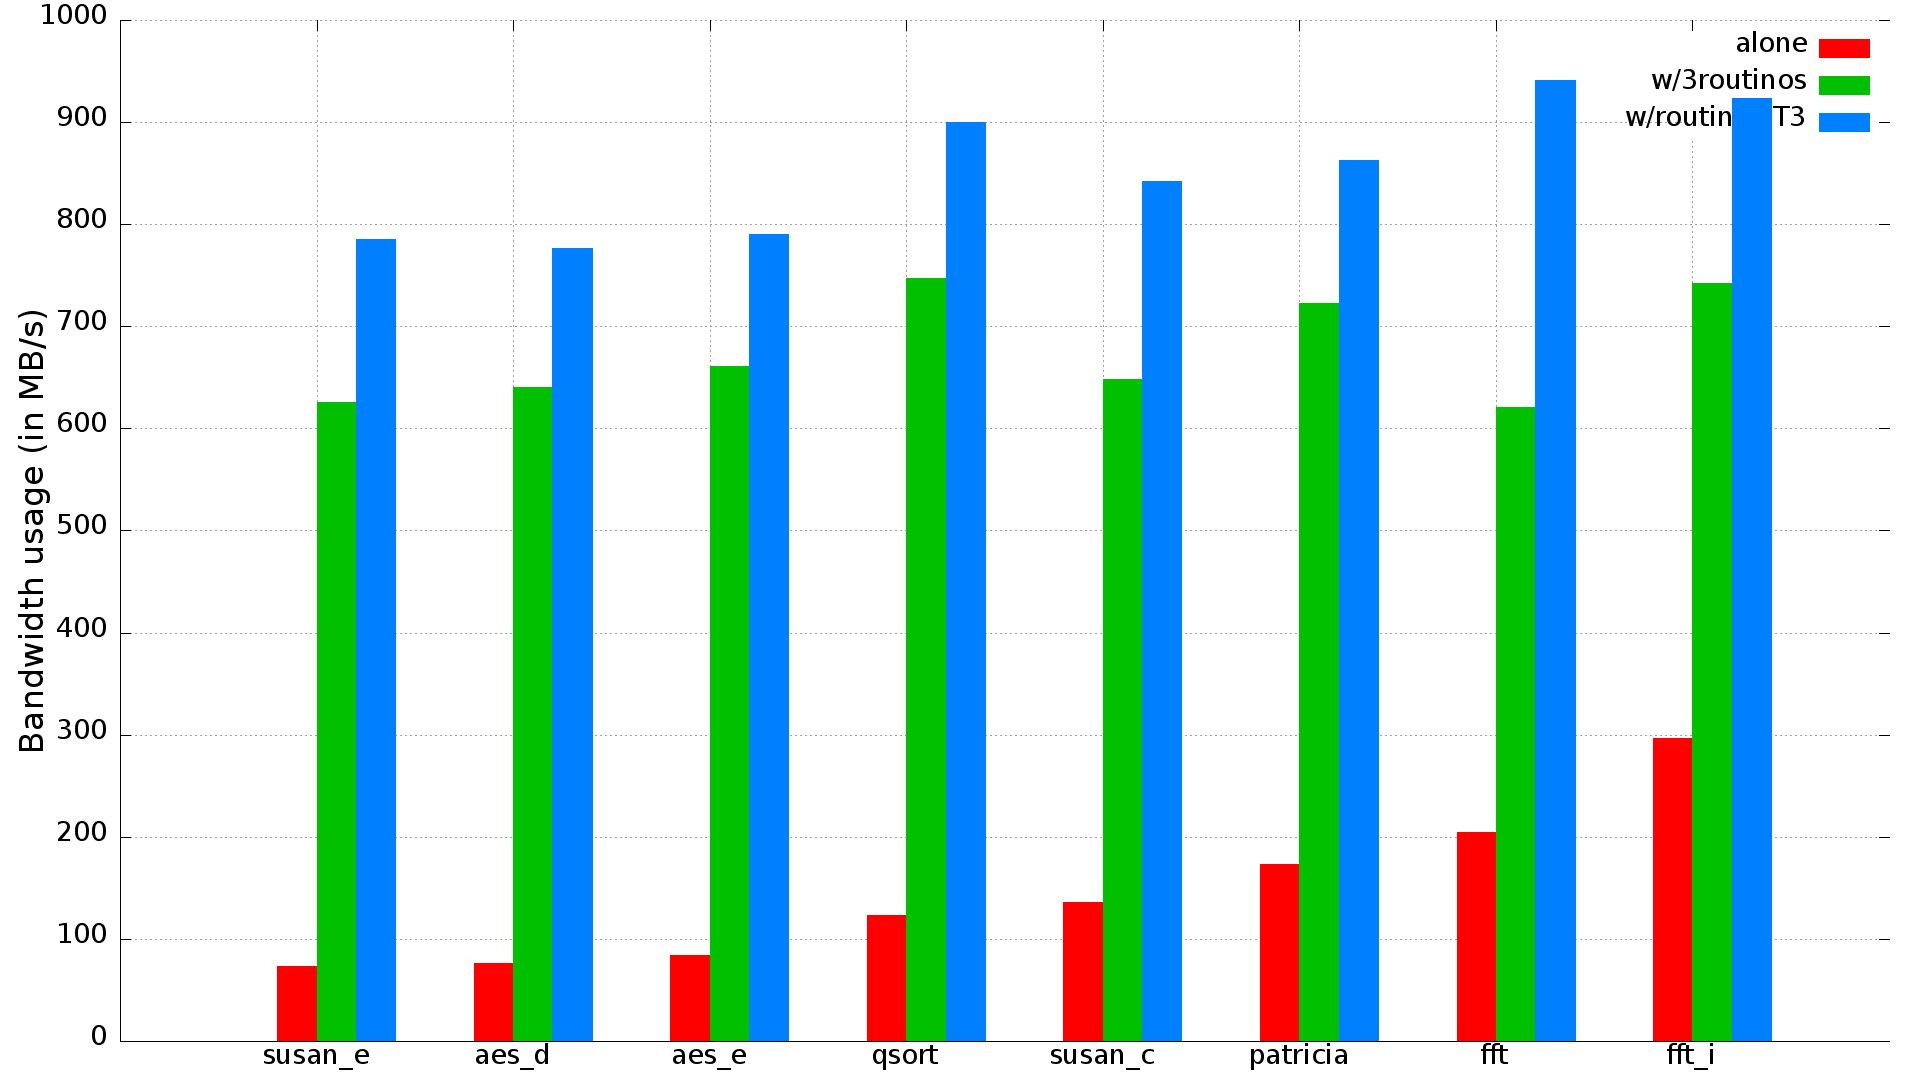
\includegraphics[scale=0.175]{include/bandwidth.png}
  \end{center}
  \visible<2>{
    \begin{exampleblock}{Observations}
      La bande passante utilisée est similaire pour toutes les tâches du 
      benchmark. Les différences sont notamment dûes aux durées d'exécution
      de chacune.
    \end{exampleblock}
  }
\end{frame}

%------------------------------------------------

\begin{frame}
  \frametitle{\'Etude d'impact sur une tâche temps-réel}
  \framesubtitle{Corrélation bande passante/overhead}
  \begin{center}
    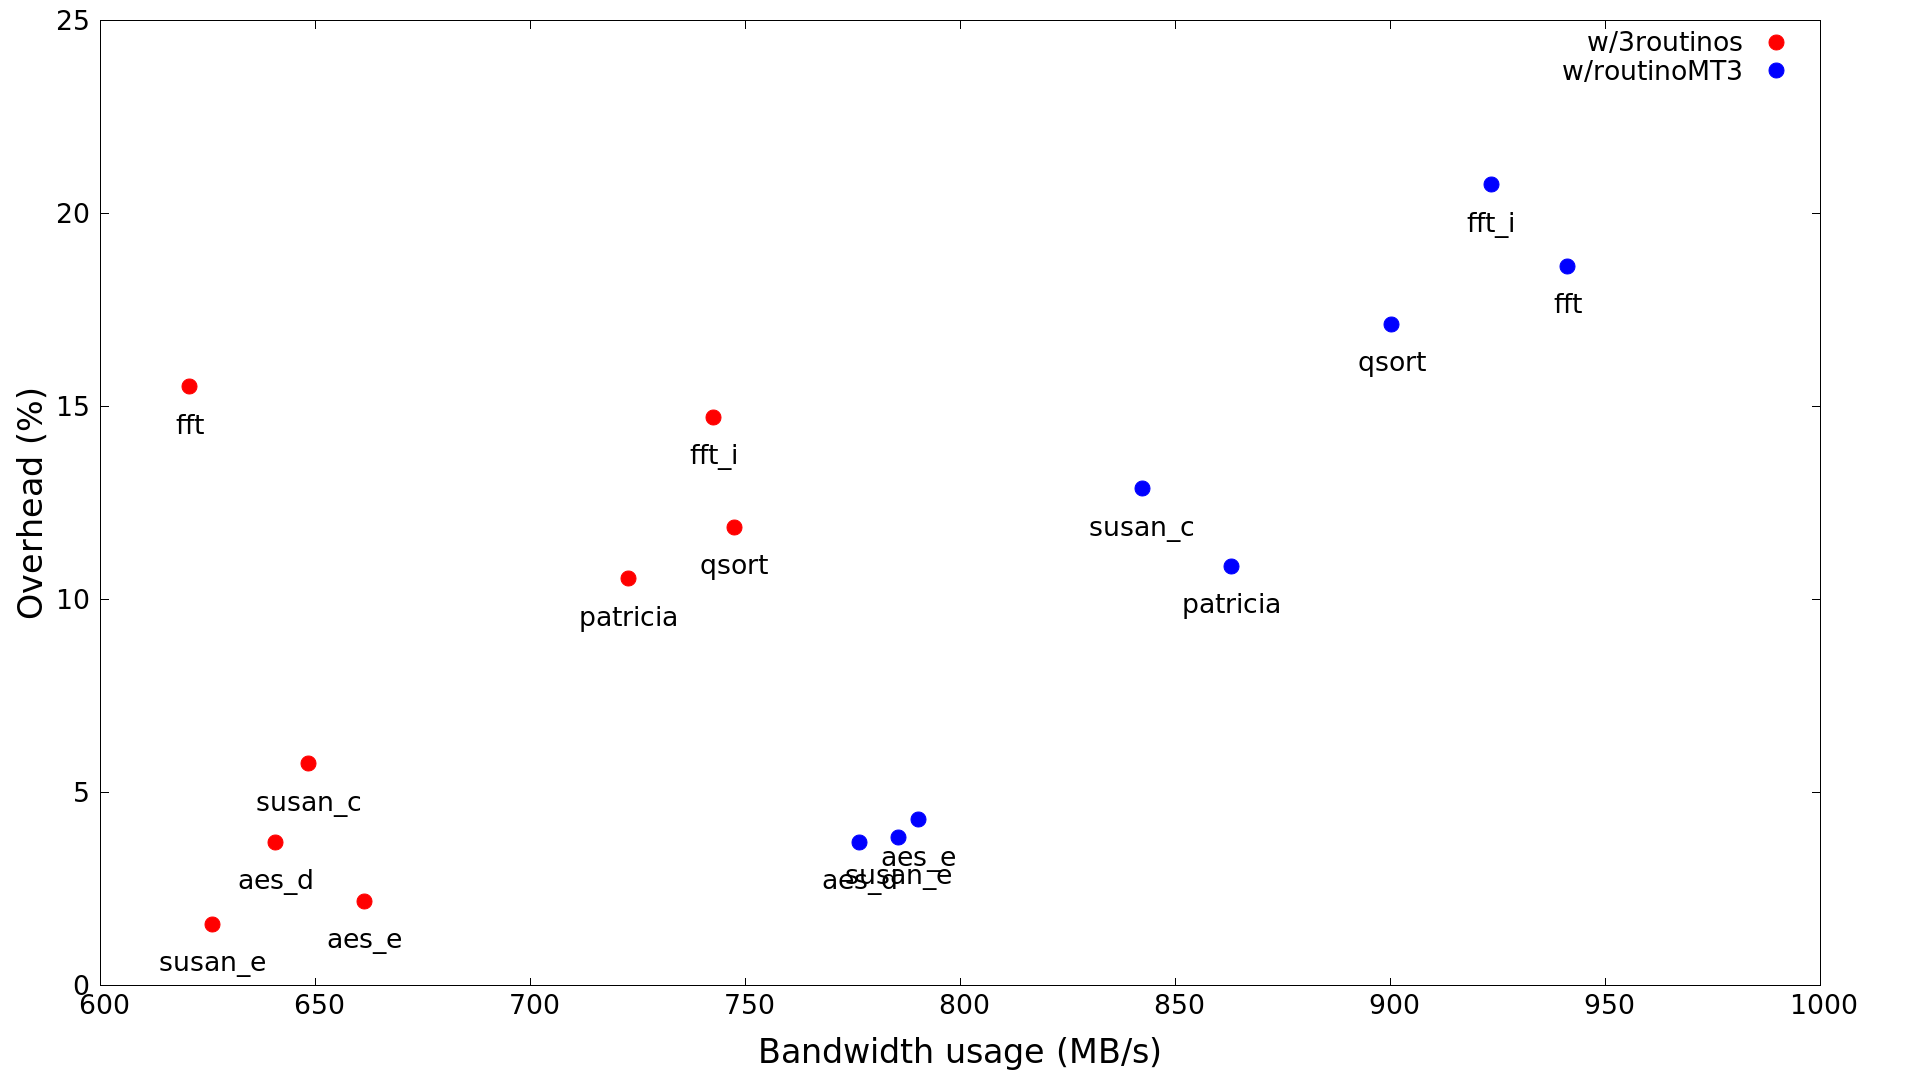
\includegraphics[scale=0.14]{include/correl.png}
  \end{center}
  \visible<2>{
    \begin{exampleblock}{Observation}
      Progression de l'overhead quasi-linéaire pour chaque type
      d'exécution (avec 3 instances de Routino ou avec RoutinoMT sur 3 threads)
    \end{exampleblock}
  }
\end{frame}

%------------------------------------------------

%---------------------------------------------------------------------------
